\subsection*{Somme de contrôle}

\begin{frame}{Somme de contrôle : définition}
  \begin{block}{Définition : somme de contrôle}
    Une somme de contrôle est une petite quantité de données additionnelle qui est calculée à partir d'un ensemble plus large de données. Elle est utilisée pour vérifier l'intégrité des données et détecter les erreurs ou les altérations éventuelles.
  \end{block}

  Exemples :

  \begin{itemize}
    \item Numéro de sécurité sociale
    \item Numéro de carte bancaire
    \item IBAN
    \item Mémoire ECC (Error Correcting Code)
  \end{itemize}
\end{frame}

\begin{frame}[fragile]{Somme de contrôle : exemple du numéro de sécurité sociale}
  Les deux derniers chiffres du numéro de sécurité sociale ne contiennent aucune information mais ils sont utilisés comme somme contrôle, pour limiter les risques de faute d'erreur.

  La formule permettant de calculer la clé est la suivante :

  $$
    \textrm{clé} = 97 - NIR \bmod 97
  $$

  $$
    \underbrace{2 69 05 49 588 157}_{\textrm{numéro NIR}}\underbrace{80}_{\textrm{clé}}
  $$

  \begin{minted}{text}
      >>> 97 - 2690549588157 % 97
      80
    \end{minted}
\end{frame}

\begin{frame}{Somme de contrôle : exemple de l'ISBN}
  L'ISBN-13 (International Standard Book Number) utilise une somme de contrôle pour détecter les erreurs de saisie :

  \begin{itemize}
    \item Chaque chiffre est multiplié alternativement par 1 et 3
    \item La somme est calculée
    \item Le dernier chiffre est choisi pour que la somme soit divisible par 10
  \end{itemize}

  Exemple avec ISBN : 978-2-1234-5680-\textbf{3}
  
  $$(9\times1 + 7\times3 + 8\times1 + 2\times3 + 1\times1 + 2\times3 + 3\times1 + 4\times3 + 5\times1 + 6\times3 + 8\times1 + 0\times3 + \textbf{3}\times1) \bmod 10 = 0$$
\end{frame}

\begin{frame}{Somme de contrôle : codes-barres UPC}
  Le code UPC (Universal Product Code) à 12 chiffres utilise une somme de contrôle :

  \begin{enumerate}
    \item Additionner les chiffres en position impaire $\times 3$
    \item Additionner les chiffres en position paire
    \item La somme de contrôle complète à $10$
  \end{enumerate}

  \begin{center}
    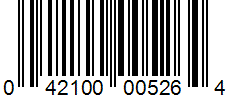
\includegraphics[width=0.5\textwidth]{img/upc-barcode.png}
    
    Exemple : 042100005264
  \end{center}
\end{frame}
